%==================================================
%
% Copyright (c) 2016 Université de Lorraine & Luleå tekniska universitet
% Author: Luca Di Stasio <luca.distasio@gmail.com>
%                       <luca.distasio@ingpec.eu>
%
% This program is free software: you can redistribute it and/or modify
% it under the terms of the GNU General Public License as published by
% the Free Software Foundation, either version 3 of the License, or
% (at your option) any later version.
%
% This program is distributed in the hope that it will be useful,
% but WITHOUT ANY WARRANTY; without even the implied warranty of
% MERCHANTABILITY or FITNESS FOR A PARTICULAR PURPOSE.  See the
% GNU General Public License for more details.
%
% You should have received a copy of the GNU General Public License
% along with this program.  If not, see <http://www.gnu.org/licenses/>.
%
%==================================================

%----------------------------------------------------------------------------------------------%
%                                 		Document class
%----------------------------------------------------------------------------------------------%

\documentclass[final]{beamer}

%----------------------------------------------------------------------------------------------%
%                                 Packages and basic declarations
%----------------------------------------------------------------------------------------------%

%\usepackage{adjustbox}
\usepackage{amsmath}
\usepackage{amssymb}
\usepackage{amsthm}
\usepackage{booktabs}
\usepackage[english]{babel}
\usepackage[orientation=landscape,size=a0,scale=1.]{beamerposter}
\usepackage{graphicx}
\usepackage[latin1]{inputenc}
\usepackage{latexsym}
\usepackage{makecell}
\usepackage{multirow}
\usepackage{ocgx}
\usepackage{tabularx}
\usepackage{tikz}

\usetikzlibrary{arrows}



%----------------------------------------------------------------------------------------------%
%                                	      Color definition
%----------------------------------------------------------------------------------------------%

%----------------------------------------------------------------------------------------------%
%                                	   Template definition
%----------------------------------------------------------------------------------------------%

\setbeamertemplate{headline}{  

\begin{table}
\begin{tabularx}{0.975\paperwidth}{lXr}
&&\\[30pt]
\makecell{
\includegraphics[width=0.15\paperwidth]{lulea_logo1}} & \makecell{\usebeamercolor{title in headline}{\centering\color{fg}\textbf{\huge{\inserttitle}}}\\[40pt]\usebeamercolor{author in headline}{\centering\color{fg}\LARGE{\insertauthor}}\\ [30pt]\usebeamercolor{institute in headline}{\centering\color{fg}\Large{$^{1}$ \'Ecole Europ\'eenne d'Ing\'enieurs en G\'enie des Mat\'eriaux, Universit\'e de Lorraine, Nancy, France}}\\ [20pt]\usebeamercolor{institute in headline}{\centering\color{fg}\Large{$^{2}$ Avdelningen f\"or materialvetenskap, Lule\aa\ tekniska universitet, Lule\aa , Sverige}}\\} &\makecell{
\includegraphics[width=0.175\paperwidth]{erasmusmundus_logo}}


% \usebeamercolor{title in headline}{\centering\color{fg}\textbf{\huge{\inserttitle}}}& \multirow{4}{*}{\centering\arraybackslash\adjustbox{valign=c}{
\includegraphics[width=0.15\paperwidth]{erasmusmundus_logo}}}\\ [40pt]
%&\usebeamercolor{author in headline}{\centering\color{fg}\LARGE{\insertauthor}}& \\ [30pt]
% &\usebeamercolor{institute in headline}{\centering\color{fg}\Large{$^{1}$ \'Ecole Europ\'eenne d'Ing\'enieurs en G\'enie des Mat\'eriaux, Universit\'e de Lorraine, Nancy, France}}& \\ [20pt]
% &\usebeamercolor{institute in headline}{\centering\color{fg}\Large{$^{2}$ Avdelningen f\"or materialvetenskap, Lule\aa\ tekniska universitet, Lule\aa , Sverige}}& \\
\end{tabularx}

\end{table}
}


\setbeamertemplate{footline}{
\begin{table}
\begin{tabularx}{0.975\paperwidth}{cXr}
&&\\[30pt]
\makecell{
\includegraphics[width=0.09\paperwidth]{Docmase_logo}} & \makecell{\usebeamercolor{institute in headline}{\centering\color{fg}\Large{\textbf{Aknowledgements}}}\\ [20pt]\usebeamercolor{institute in headline}{\centering\color{fg}\Large{The authors wish to thank}}\\} &\makecell{
\includegraphics[width=0.2\paperwidth]{logo-eeigm}}


\end{tabularx}

\end{table}
}

%----------------------------------------------------------------------------------------------%
%                                	        Data definition
%----------------------------------------------------------------------------------------------%

\title{2D Representative Volume Elements for Intralaminar Damage Modeling in FRPCs}
%\author{\href{http://www.lucadistasioengineering.com}{Luca Di~Stasio}}
%\institute[Universit\'e de Lorraine]{Department of Computer Science, Drexel University, Philadelphia, PA, USA}
\author{Luca Di Stasio \inst{1,2} \and Zoubir Ayadi \inst{1} \and Janis Varna \inst{2}}
%\institute{\inst{1} \'Ecole Europ\'eenne d'Ing\'enieurs en G\'enie des Mat\'eriaux, Universit\'e de Lorraine, Nancy, France \and %
%                      \inst{2} Avdelningen f\"or materialvetenskap, Lule\aa\ tekniska universitet, Lule\aa , Sverige}
\date{\today}

\graphicspath{{./pics/}}

\beamertemplatenavigationsymbolsempty

%----------------------------------------------------------------------------------------------%
%----------------------------------------------------------------------------------------------%
%                                            DOCUMENT STARTS
%----------------------------------------------------------------------------------------------%
%----------------------------------------------------------------------------------------------%

\begin{document}

\begin{frame}
\begin{tabularx}{0.975\paperwidth}{cccc|c ccccc ccccc ccccc ccccc ccccc ccccc ccccc ccccc ccccc ccccc ccccc ccccc ccccc ccccc ccccc cccc}% 84 columns
&&&&\multicolumn{20}{c}{Traction/Compression}&\multicolumn{20}{c}{Flexion}&\multicolumn{20}{c}{In-plane Shear}&\multicolumn{20}{c}{Out-of-Plane Shear}\\
&&&&\multicolumn{10}{c}{Displacement controlled}&\multicolumn{10}{c}{Force controlled}&\multicolumn{10}{c}{Displacement controlled}&\multicolumn{10}{c}{Force controlled}&\multicolumn{10}{c}{Displacement controlled}&\multicolumn{10}{c}{Force controlled}&\multicolumn{10}{c}{Displacement controlled}&\multicolumn{10}{c}{Force controlled}\\
\midrule
\multirow{5}{*}{\rotatebox[origin=c]{90}{2D}}&\multirow{4}{*}{\rotatebox[origin=c]{90}{Single RVE}}&\multirow{2}{*}{\rotatebox[origin=c]{90}{Single Fiber}}&\rotatebox[origin=c]{90}{Single Crack}&\begin{ocg}{Image A}{ocg1}{1}\actionsocg{}{ocg2}{ocg1}{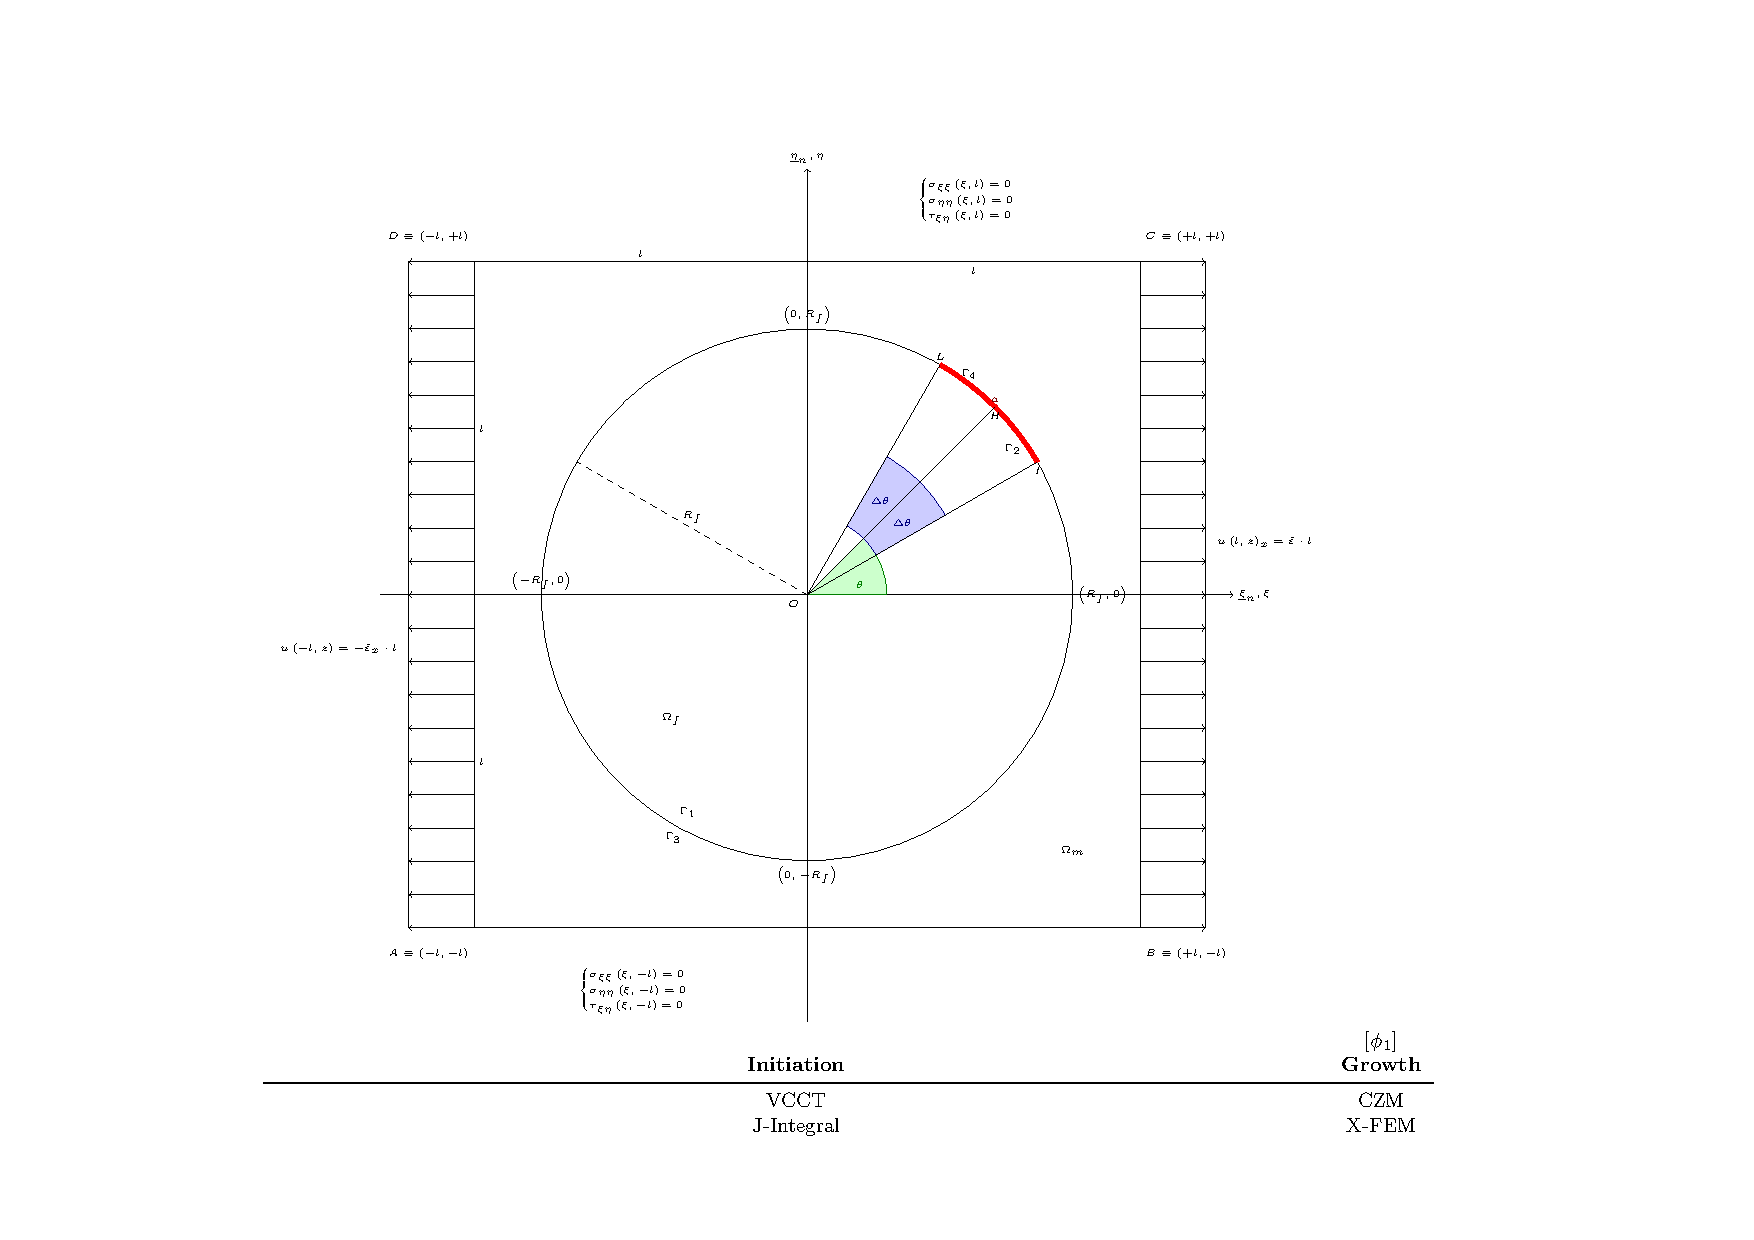
\includegraphics[width=0.1\textwidth]{./elements/ELEMENT-A-A.pdf}}\end{ocg}\begin{ocg}{Image B}{ocg2}{0}\actionsocg{}{ocg1}{ocg2}{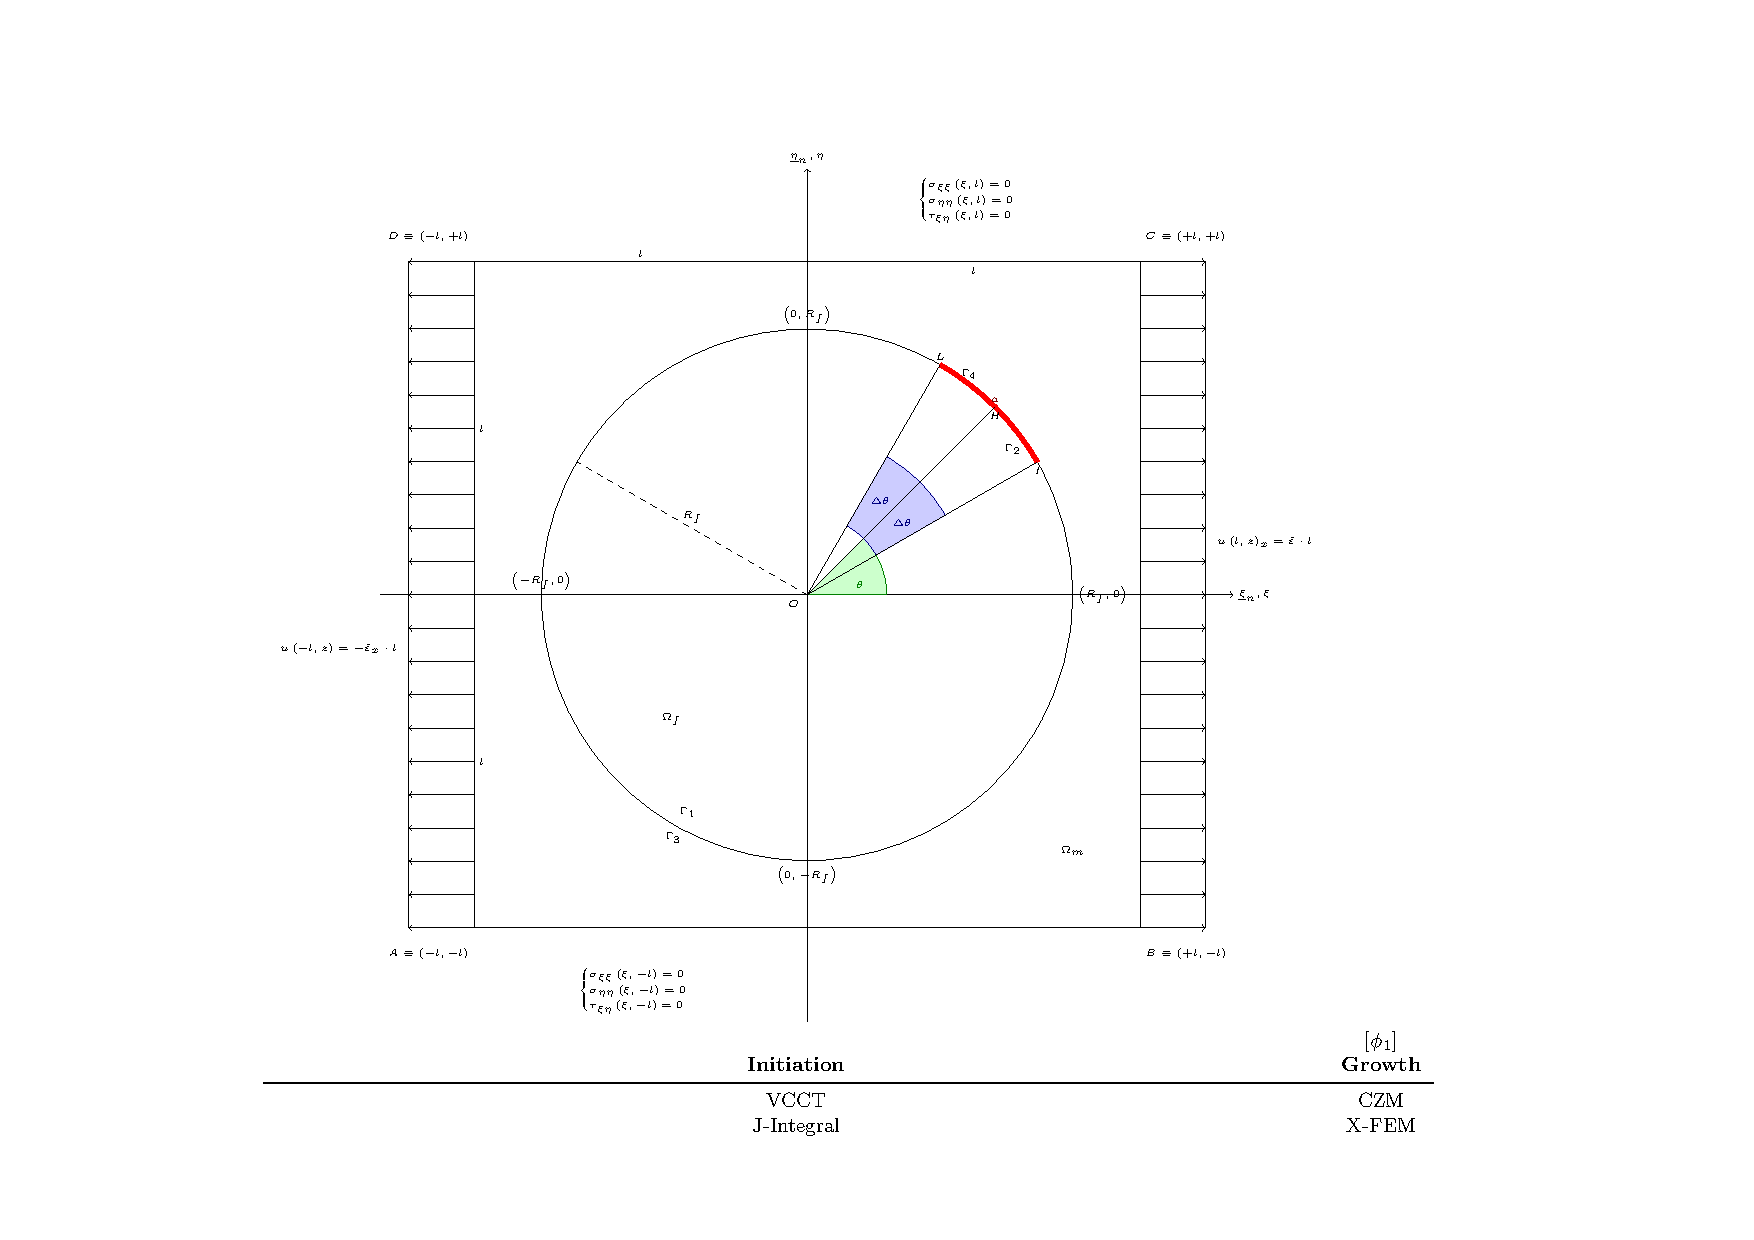
\includegraphics[width=\textwidth]{./elements/ELEMENT-A-A.pdf}}\end{ocg}&\multicolumn{79}{c}{we're working for you}\\
&&&\rotatebox[origin=c]{90}{Multiple Cracks}&\multicolumn{80}{c}{we're working for you}\\
&&\multirow{2}{*}{\rotatebox[origin=c]{90}{Multiple Fibers}}&\rotatebox[origin=c]{90}{Single Crack}&\multicolumn{80}{c}{we're working for you}\\
&&&\rotatebox[origin=c]{90}{Multiple Cracks}&\multicolumn{80}{c}{we're working for you}\\
&\rotatebox[origin=c]{90}{Multiple RVEs}&&&\multicolumn{80}{c}{we're working for you}\\
&\rotatebox[origin=c]{90}{Experimental Settings}&&&\multicolumn{80}{c}{we're working for you}\\
%\midrule
%\multirow{5}{*}{\rotatebox[origin=c]{90}{Quasi-3D}}&\multirow{4}{*}{\rotatebox[origin=c]{90}{Single RVE}}&\multirow{2}{*}{\rotatebox[origin=c]{90}{Single Fiber}}&\rotatebox[origin=c]{90}{Single Debond}&\multicolumn{80}{c}{we're working for you}\\
%&&&\rotatebox[origin=c]{90}{Multiple Debonds}&\multicolumn{80}{c}{we're working for you}\\
%&&\multirow{2}{*}{\rotatebox[origin=c]{90}{Multiple Fibers}}&\rotatebox[origin=c]{90}{Single Debond}&\multicolumn{80}{c}{we're working for you}\\
%&&&\rotatebox[origin=c]{90}{Multiple Debonds}&\multicolumn{80}{c}{we're working for you}\\
%&\rotatebox[origin=c]{90}{Multiple RVEs}&&&\multicolumn{80}{c}{we're working for you}\\
%&\rotatebox[origin=c]{90}{Experimental Settings}&&&\multicolumn{80}{c}{we're working for you}\\
%\midrule
%\multirow{5}{*}{\rotatebox[origin=c]{90}{3D}}&\multirow{4}{*}{\rotatebox[origin=c]{90}{Single RVE}}&\multirow{2}{*}{\rotatebox[origin=c]{90}{Single Fiber}}&\rotatebox[origin=c]{90}{Single Debond}&\multicolumn{80}{c}{we're working for you}\\
%&&&\rotatebox[origin=c]{90}{Multiple Debonds}&\multicolumn{80}{c}{we're working for you}\\
%&&\multirow{2}{*}{\rotatebox[origin=c]{90}{Multiple Fibers}}&\rotatebox[origin=c]{90}{Single Debond}&\multicolumn{80}{c}{we're working for you}\\
%&&&\rotatebox[origin=c]{90}{Multiple Debonds}&\multicolumn{80}{c}{we're working for you}\\
%&\rotatebox[origin=c]{90}{Multiple RVEs}&&&\multicolumn{80}{c}{we're working for you}\\
%&\rotatebox[origin=c]{90}{Experimental Settings}&&&\multicolumn{80}{c}{we're working for you}\\
\end{tabularx}
\end{frame}

\end{document}